\section{Datenbearbeitung im Internet}

\subsection{Datenschutz}
\begin{itemize}
    \item \textbf{Datenschutz}
    \begin{itemize}
        \item Schutz der Persönlichkeit und der Grundrechte der Personen, über die Daten bearbeitet werden
    \end{itemize}
    \item \textbf{Personendaten} (Daten)
    \begin{itemize}
        \item alle Angaben, die sich auf eine bestimmte oder bestimmbare Person beziehen
        \item Adresse, Vor-/Nachname, Geburtsdatum, IP-Adresse etc.
    \end{itemize}
    \item \textbf{Datenbearbeitung}
    \begin{itemize}
        \item Eingriff in Persönlichkeitsrechte
        \item Datenbearbeitung ohne Rechtfertigungsgrund ist ein widerrechtlicher Eingriff ins Persönlichkeitsrecht
    \end{itemize}
\end{itemize}

\subsubsection{Datenschutz EU/ Schweiz}
\begin{minipage}{0.5\linewidth}
    \paragraph{Europa}
    \begin{itemize}
        \item Richtlinie Europarat/Schengen
        \item EU-Datenschutz-Grundverordnung (DSGVO) / nationale Datenschutzgesetze
    \end{itemize}
\end{minipage}
\begin{minipage}{0.5\linewidth}
    \paragraph{Schweiz}
    \begin{itemize}
        \item Richtlinie Europarat/Schengen
        \item DSG / kantonale Datenschutzgesetze\\
    \end{itemize}
\end{minipage}
$\rightarrow$ zur Zeit gleichwertiges Datenschutzniveau!!

\subsubsection{Datenschutz USA/ Schweiz}
\begin{minipage}{0.5\linewidth}
    \paragraph{USA}
    \begin{itemize}
        \item Datenschutzgesetze in einzelnen Bundesstaaten, jedoch kein nat. Datenschutzgesetz
        \item Selbstregulierung (Privacy Policies von Unternehmen)
    \end{itemize}
\end{minipage}
\begin{minipage}{0.5\linewidth}
    \paragraph{Schweiz}
    \begin{itemize}
        \item Richtlinie Europarat/Schengen
        \item DSG / kantonale Datenschutzgesetze\\
    \end{itemize}
\end{minipage}
$\rightarrow$ zur Zeit nicht gleichwertiges Datenschutzniveau!!

\subsection{Rechtfertigungsgründe}
\begin{itemize}
    \item Einwilligung der betroffenen Person
    \item überwiegendes privates oder öffentliches Interesse
    \item gesetzliche Grundlage
\end{itemize}

\subsection{Rechte der betroffenen Person}
\begin{minipage}{0.5\linewidth}
    \paragraph{nach Datenschutzgesetz}
    \begin{itemize}
        \item Auskunftsrecht
        \item Sperr-, Korrektur-, Löschungsrecht
    \end{itemize}
    \paragraph{nach Zivilrecht}
    \begin{itemize}
        \item Persönlichkeitsverletzung (ZGB)
        \item Schadenersatz / Genugtuung (OR)
    \end{itemize}
\end{minipage}
\begin{minipage}{0.5\linewidth}
    \paragraph{nach Strafrecht (StGB)}
    \begin{itemize}
        \item unbefugte Datenbeschaffung
        \item unbefugtes Eindringen in eine Datenverarbeitungsanlage
        \item Datenbeschädigung
        \item Datenbeschädigung
    \end{itemize}
\end{minipage}

\subsection{Datenschutzrechtliche Grundprinzipien}
\begin{itemize}
    \item Rechtfertigung
    \item Zweckgebundenheit
    \item Verhältnismässigkeit
    \item Integrität
    \item Sicherheit (AV aktuell, FW vorhanden, etc.)
    \item Transparenz
    \item Verantwortung (Online Shop kann Haftbar gemacht werden)
\end{itemize}

\subsection{Datenschutzgesetze}
\begin{minipage}{0.5\linewidth}
    \paragraph{Bund}
    \begin{itemize}
        \item Bundesgesetz über den Datenschutz (DSG)
    \end{itemize}
    \paragraph{Geltungsbereich}
    \begin{itemize}
        \item Privatpersonen + private Unternehmungen
        \item Bundesorgane
    \end{itemize}
\end{minipage}
\begin{minipage}{0.5\linewidth}
    \paragraph{Kantone}
    \begin{itemize}
        \item eigene Datenschutzgesetze
    \end{itemize}
    \paragraph{Geltungsbereich}
    \begin{itemize}
        \item öffentliche Organe auf kantonaler und kommunaler Ebene
        \item mit öffentlichen Aufgaben betraute Private
    \end{itemize}
\end{minipage}

\subsection{Personalisierung im Onlinemarketing}
\begin{itemize}
    \item Personal Pricing
    \begin{itemize}
        \item Angebot / Preis richtet sich nach Kaufkraft des Käufers (Bsp. Flugtickets in CH teurer als in IT)
        \item Rechtlich Gesehen befindet man sich gemäss der Schweizer Gesetzgebung in einem "Graubereich"
    \end{itemize}
    \item Kollaboratives Filtern
    \begin{itemize}
        \item Empfehlungen gestützt auf Nutzungsverhalten anderer Nutzer (Bsp. Amazon)
    \end{itemize}
    \item Technologien
    \begin{itemize}
        \item Data-Mining, Filtertechnologien, Cookies, Beacon, Augmented Reality
    \end{itemize}
\end{itemize}

\subsection{Anmeldung Datensammlung}
DSG verpflichtet Privatpersonen zur Anmeldung von Datensammlungen beim EDÖB falls
\begin{itemize}
    \item regelmässig besonders schützenswerte Personendaten oder Persönlichkeitsprofile bearbeitet werden oder
    \item regelmässig Personendaten an Dritte bekannt gegeben werden
\end{itemize}

\subsection{Datensicherheit}
\begin{center}
    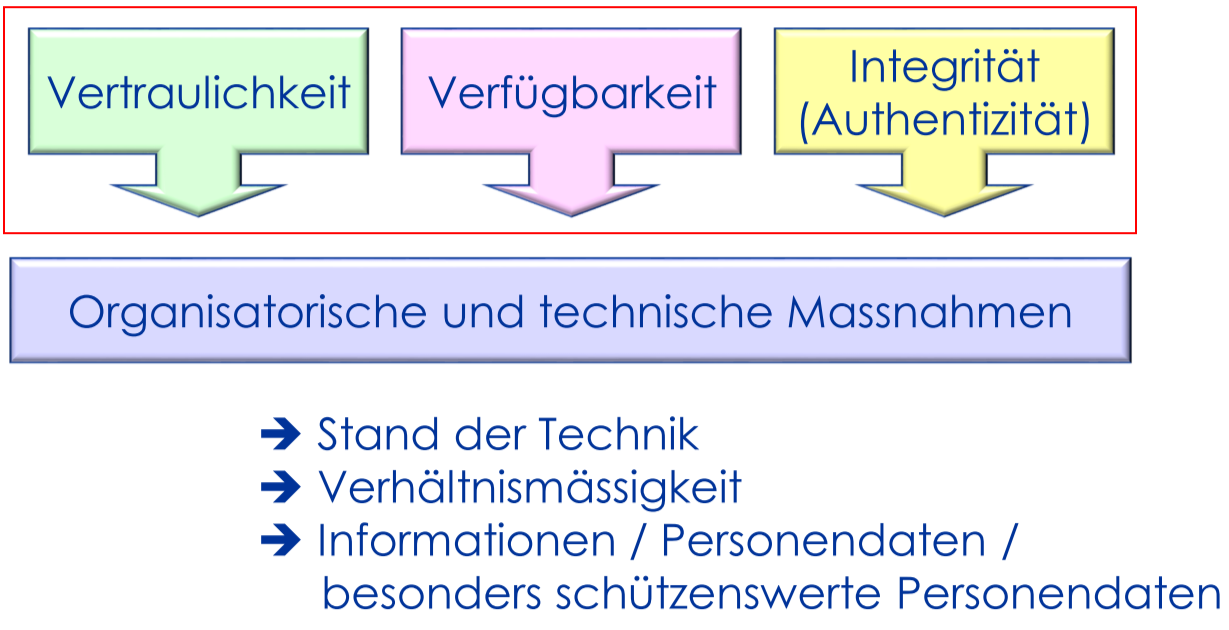
\includegraphics[width=0.8\linewidth]{01-datenbearbeitung/01-datensicherheit}
\end{center}
\textcolor{red}{\textbf{Datensicherheit ist wichtigstes Grundprinzip für Online Shops!!}}

\subsection{Privacy Policy}
\begin{itemize}
    \item Privacy Policy = Datenbearbeitungserklärung
    \begin{itemize}
        \item orientiert darüber, nach welchen (selbst auferlegten) Prinzipien ein Unternehmen Personendaten (insbesondere von Kunden) bearbeitet
    \end{itemize}
\end{itemize}

\subsubsection{Grenzüberschreitende Bekanntgabe}
DSG verlangt angemessenen Schutz von ins Ausland übermittelten Daten durch
\begin{itemize}
    \item genügende Gesetzgebung im Zielland oder anderweitige Massnahmen
    \item $\rightarrow$ hinreichende vertragliche Garantien des Empfängers
    \item $\rightarrow$ Verschlüsselung oder Pseudo- bzw. Anonymisierung
\end{itemize}